\documentclass[conference]{IEEEtran}
\usepackage{booktabs}
\usepackage{graphicx}
\usepackage{microtype}
\usepackage{siunitx}
\usepackage{url}

\graphicspath{{../results/figures/}}
\sisetup{detect-all}

\title{When Better Prediction Does Not Reliably Improve Trading:
A Reproducible ANN--MPS Evaluation in FinRL}

\author{\IEEEauthorblockN{Aarav Nagar}}

\begin{document}
\maketitle

\begin{abstract}
Quantum-inspired tensor networks can provide compact predictive
representations, but lower prediction error need not improve a sequential
trading policy. We evaluate a classically simulated matrix product state (MPS)
return signal against an artificial neural network (ANN) signal and the
standard FinRL state under matched Proximal Policy Optimization (PPO)
conditions. The protocol separates representation validation from downstream
policy evaluation, prespecifies PPO-budget and MPS-capacity selection, and
retains negative or unstable results. A three-seed capacity pilot found all
tested MPS bond dimensions within one percent validation mean-squared error;
the frozen parsimony rule selected bond dimension two (97 parameters).
Pilot trading differences changed across seeds and did not establish a stable
MPS advantage. The primary ten-seed comparison and shifted-period robustness
analysis are intentionally withheld from this draft until their validated,
hash-linked artifacts complete.
\end{abstract}

\begin{IEEEkeywords}
FinRL, matrix product state, tensor network, proximal policy optimization,
quantum-inspired machine learning, reproducibility
\end{IEEEkeywords}

\section{Introduction}

Financial reinforcement learning couples noisy predictive information to a
policy that must act under costs, path dependence, and changing market
conditions. FinRL provides a layered framework for constructing and evaluating
such trading agents \cite{liu2020finrl}, while PPO offers a widely used
clipped-policy-gradient objective \cite{schulman2017ppo}. These ingredients make
downstream portfolio behavior, rather than prediction error alone, the
appropriate endpoint for a trading representation.

Tensor networks have been proposed as compact, quantum-inspired supervised
models \cite{stoudenmire2016supervised}. They are related to broader quantum
machine-learning research \cite{biamonte2017quantum}, but a classical tensor
network does not imply quantum execution or quantum advantage. This paper asks
whether an MPS next-day-return signal improves out-of-sample PPO trading
relative to an ANN signal when data, costs, policy architecture, random seeds,
and training budget are held fixed.

Our contribution is an evidence-linked evaluation that (i) separates
representation selection from trading outcomes, (ii) prespecifies capacity and
training-budget decisions, (iii) uses matched policy seeds and paired
uncertainty summaries, and (iv) reports null, negative, or unstable outcomes
without reframing them as an advantage.

\section{Related Work}

PPO alternates data collection with multiple epochs of minibatch optimization
while constraining policy changes through a clipped surrogate objective
\cite{schulman2017ppo}. FinRL adapts deep reinforcement-learning algorithms,
market environments, and evaluation tooling to automated trading
\cite{liu2020finrl}. Quantum-inspired tensor-network models instead factorize a
high-order representation into locally connected tensors, offering a capacity
control distinct from a dense ANN \cite{stoudenmire2016supervised}. Prior work
on quantum tensor networks for variational reinforcement learning motivates
studying the interface between tensor representations and policy learning
\cite{liu2020quantumtensor}; our experiment remains wholly classical.

\section{Methods}

\subsection{Data and temporal separation}

The experiment uses 15 Nasdaq stocks from a saved, checksum-verified processed
dataset. Encoder fitting uses 2013--2017 observations, 2018 is reserved for
encoder validation and early stopping, PPO policies train on 2013--2018, and
portfolio evaluation uses 2019--2023. Neither encoder nor PPO fitting uses the
2019--2023 return target. A recorded FinRL commit and dependency lock bind the
software environment.

\subsection{Representations and state construction}

Both encoders receive 13 per-stock inputs and predict next-day return. The ANN
uses fully connected layers. The MPS maps the same inputs to a classically
contracted tensor network; its bond dimension controls capacity. The base
FinRL state contains cash, prices, holdings, and ten technical indicators for
181 values. Signal conditions append one frozen prediction per stock, producing
a 196-value state. Thus ANN and MPS policy states differ only in the final 15
values.

\subsection{Matched PPO evaluation}

Every condition uses the same two-layer, 64-unit PPO policy/value network,
initial portfolio of \$1,000,000, maximum order of 100 shares, reward scaling
of \(10^{-4}\), and 0.10\% transaction cost on executed buys and sells. A
prespecified budget pilot selected 20,000 environment steps because outcomes
and training diagnostics still changed between 10,000 and 20,000 steps; this
selection does not establish convergence.

\subsection{Capacity selection and primary estimand}

Bond dimensions 2, 4, and 8 are evaluated at the selected PPO budget using
matched pilot seeds 0--2. The frozen rule finds the minimum 2018 validation
MSE, treats configurations within 1\% as practically tied, and chooses the
fewest parameters, with fit time used only as a final tie-breaker. Test-period
prediction and trading metrics cannot select the dimension.

The primary final estimand is the mean paired MPS-minus-ANN Sharpe difference
across PPO seeds 0--9. We report every seed, the standard deviation, a
deterministic paired-seed bootstrap interval, and an exact two-sided sign test.
These quantities describe training-seed uncertainty on one historical split;
they are not causal or population-level intervals.

\section{Capacity Pilot}

All three capacity configurations fell within 1\% of the minimum validation
MSE (Table~\ref{tab:capacity}). The frozen rule selected bond dimension 2
because its 97 parameters were fewer than the 369 and 1,441 parameters of
dimensions 4 and 8. The longer measured fit time for dimension 2 did not enter
the tie-break because parameter counts differed.

\begin{table}[t]
\caption{Prespecified MPS capacity pilot}
\label{tab:capacity}
\centering
\small
\begin{tabular}{rrrr}
\toprule
Bond dim. & Parameters & Validation MSE & Fit (s) \\
\midrule
\textbf{2} & \textbf{97} & \textbf{1.280290} & \textbf{48.679} \\
4 & 369 & 1.281044 & 4.739 \\
8 & 1,441 & 1.275307 & 9.304 \\
\bottomrule
\end{tabular}
\end{table}

\begin{figure}[t]
\centering
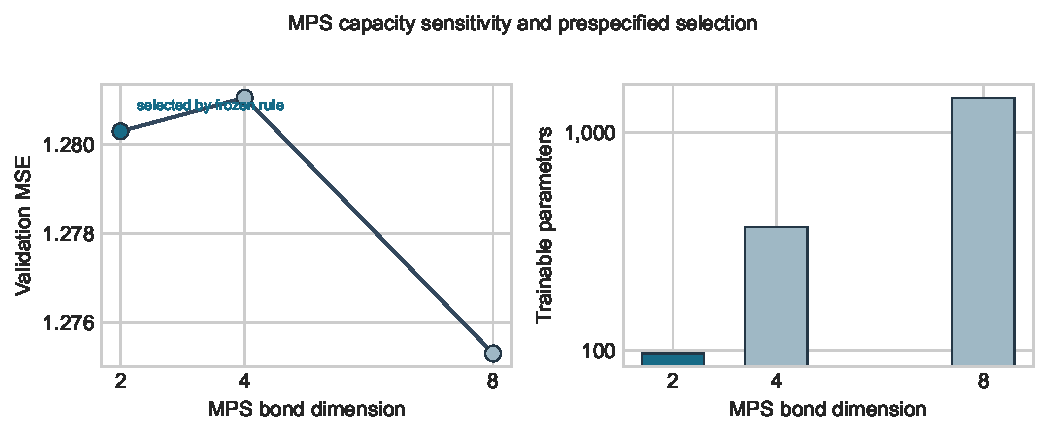
\includegraphics[width=\columnwidth]{dimension_sensitivity.pdf}
\caption{Validation MSE and parameter growth across MPS bond dimensions.
Dimension 2 is selected by the frozen validation/parsimony rule; downstream
trading outcomes do not determine selection.}
\label{fig:capacity}
\end{figure}

Mean pilot MPS-minus-ANN Sharpe differences were \(-0.045\), \(-0.027\), and
\(-0.046\) for dimensions 2, 4, and 8. Each MPS configuration exceeded ANN in
one of three matched seeds. These descriptive pilot results do not establish a
stable advantage and are not substituted for the pending ten-seed estimate.

\section{Final Evaluation and Robustness}

This section is gated on the completed ten-seed manifest, paired-effect
artifact, and shifted-period robustness evidence. Numerical placeholders are
prohibited: the submission version will populate this section only from
generated, hash-linked tables and figures registered in the claim traceability
file.

\section{Limitations}

The study uses a small 15-stock universe and one principal historical split.
The MPS is reconstructed from the stated research direction rather than an
unavailable original implementation. Capacity matching is exact only for the
reference dimension-4 ANN comparison; the selected dimension-2 model is a
parsimony-controlled sensitivity choice. PPO optimization can remain unstable
at the largest tested budget, and ten seeds still provide limited uncertainty
resolution. Backtests omit several production frictions, including market
impact, borrow constraints, and latency. Most importantly, all tensor
operations execute classically; no quantum circuit or quantum hardware is
used.

\section{Conclusion}

The current evidence supports a methodological conclusion: representation
validation, policy evaluation, and capacity selection must remain distinct.
The capacity pilot selected a compact MPS without using trading outcomes, while
its descriptive trading differences were seed-sensitive. The final conclusion
about downstream performance remains contingent on the prespecified ten-seed
and temporal-robustness artifacts.

\section*{Acknowledgment}

The author thanks Dr.\ Xiao-Yang Liu for feedback on the research direction.

\bibliographystyle{IEEEtran}
\bibliography{references}

\end{document}
